\section{Measurement of Boosted $H \rightarrow b\bar{b}$} \label{sec:results:procedure}

For the $H \rightarrow b\bar{b}$ process, the observed signal strength is:
%
$$ \mu_{H} = 5.8 \pm 3.1~\mathrm{(stat.)} \pm 1.9~\mathrm{(syst.)} \pm 1.7~\mathrm{(theo.)}\,. $$
%
Given the uncertainties, this result is consistent with the background-only
hypothesis at $1.6\sigma$ with an expected sensitivity of $0.28\sigma$
\cite{Feickert:HiggsCouplings2018}.  This constitutes a measurement of the
boosted Higgs decaying to a bottom quark pair but not a direct observation
which would require $5\sigma$. The result of the combined fit of the $V$ + jets
and $H \rightarrow b\bar{b}$ signal models agree with the Standard
Model prediction of $\mu_{H} = \mu_{V} = 1$, as seen in
\Cref{sec:results:contour}.
%
\begin{figure}
\centering
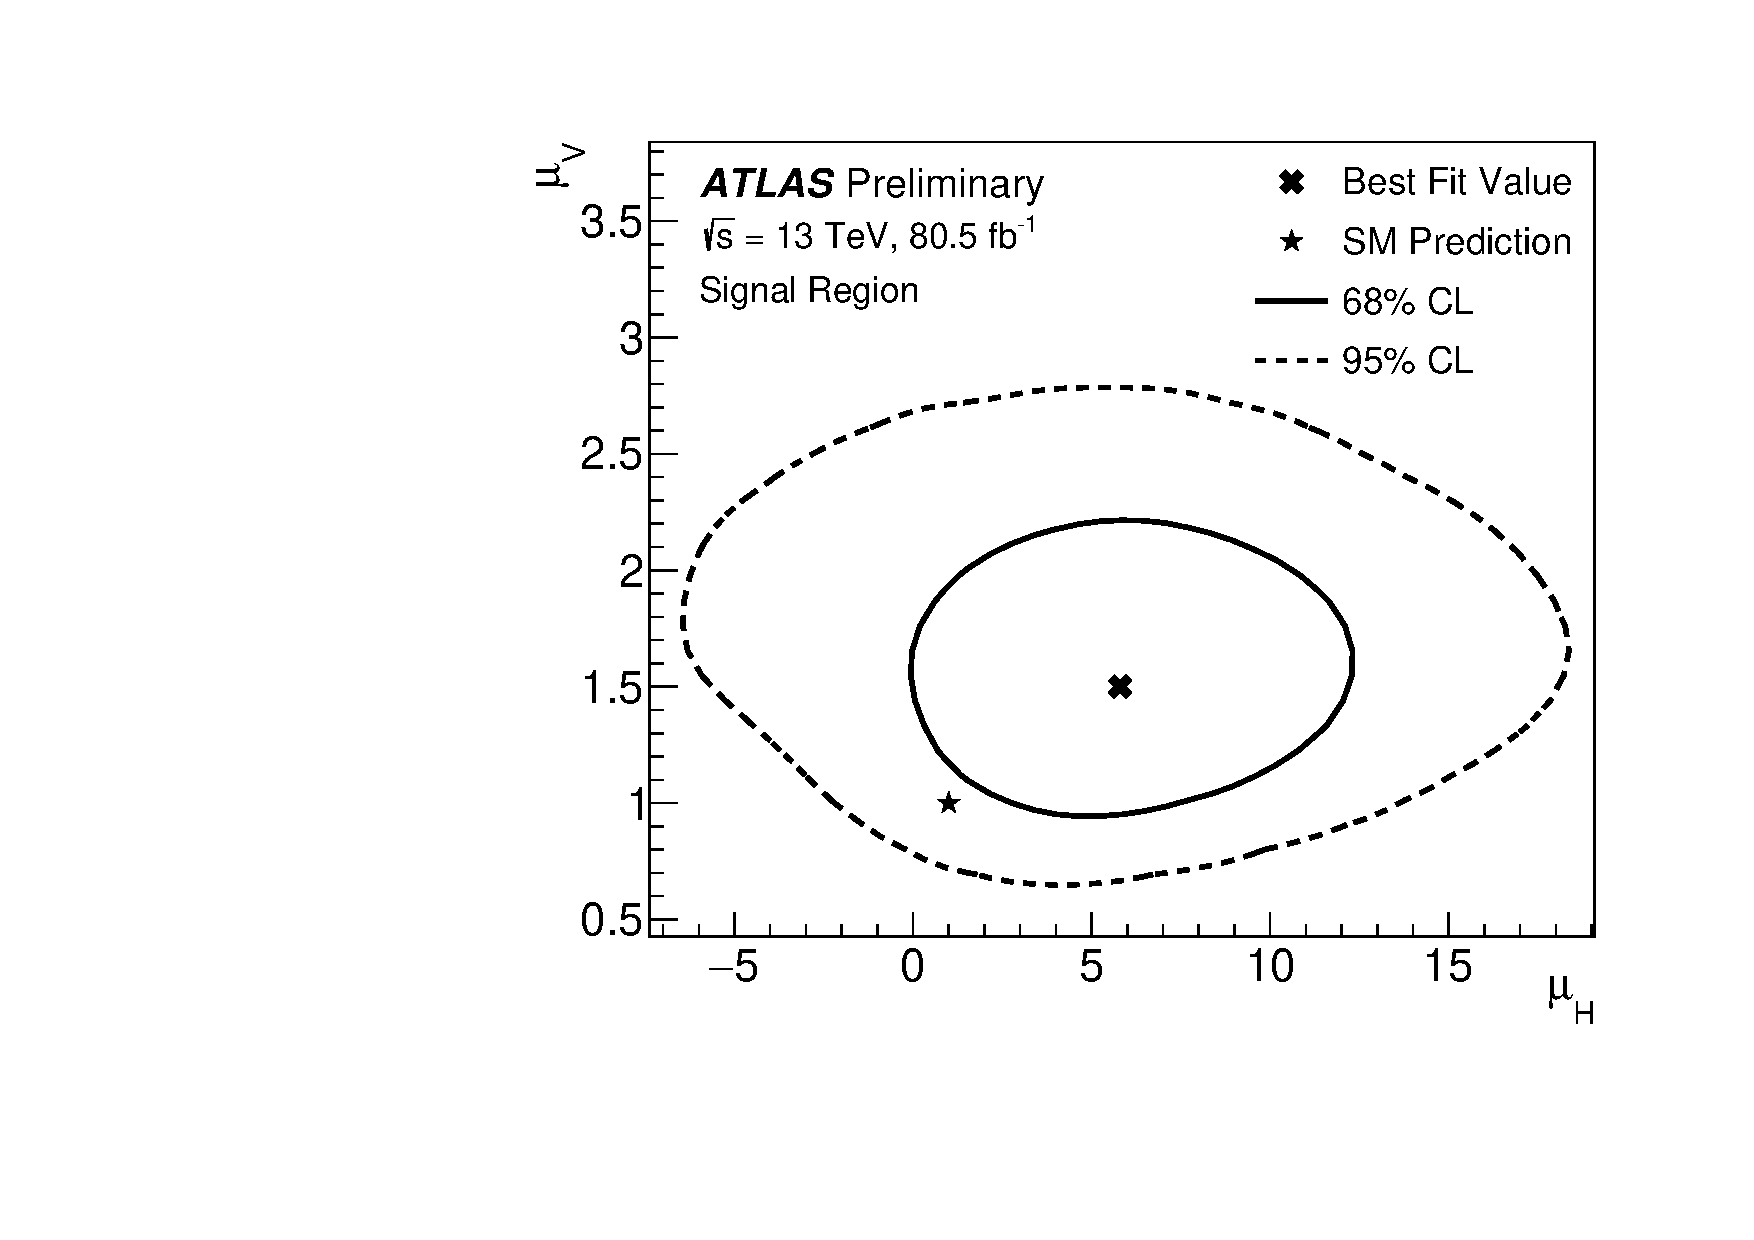
\includegraphics[width=.6\linewidth]{figures/results/contour}
\caption{
Combined marginalized posterior distributions of $\mu_{H}$ and $\mu_{V}$ in the
Signal Region \cite{ATLAS-CONF-2018-052}.  It is seen that the best-fit values for the signal processes
lie within the 68\% Credibility Level ($2\sigma$) of the Standard Model
prediction.}
\label{sec:results:contour}
\end{figure}
